\documentclass[a4j,10pt]{jarticle}
\usepackage[dvipdfm,text={160mm,240mm},centering]{geometry}
\usepackage{newtxtext,newtxmath}
\usepackage[dvipdfmx]{graphicx}
\usepackage{listings,jvlisting}
\usepackage{color}
\usepackage{tabularx}
\usepackage{booktabs}
\usepackage{multirow}
\usepackage{comment}

% 担当教員名
\newcommand{\teacherName}{桝井 晃基}
% 提出者名
\newcommand{\studentName}{鶴見 俊介}
% 提出者所属
\newcommand{\studentAff}{基礎工学部 情報科学科3年 計算機科学コース}
% 提出者学籍番号
\newcommand{\studentID}{09B23057}
% 提出者電子メールアドレス
\newcommand{\studentEmail}{u299151f@ecs.osaka-u.ac.jp}
% 課題提出日
\newcommand{\submitted}{\today}
% 課題締め切り日
\newcommand{\deadline}{2025年1月30日 23:59}

\lstset{
    basicstyle = {\ttfamily},
    backgroundcolor  = {\color[gray]{.99}},
    breaklines = true,
    columns = [l]{fullflexible},
    commentstyle = {\smallitshape},
    frame = {tb},
    identifierstyle = {\small},
    keepspaces=true,
    keywordstyle = {\small\bfseries},
    lineskip = -0.5ex,
    ndkeywordstyle = {\small},
    numbers = left,
    numbersep = 1zw,
    numberstyle = {\scriptsize},
    stepnumber = 1,
    stringstyle = {\small\ttfamily},
    xleftmargin = 3zw,
    xrightmargin = 0zw
}
\renewcommand{\lstlistingname}{プログラム}

\begin{document}
\begin{titlepage}
\begin{center}
{\Huge\bfseries 情報科学演習D} \\
\vspace{1cm}
{\LARGE\bfseries 課題4}
\vspace{5cm}

{\large
\begin{tabular}{rcl}
担当教員 & : & \teacherName \\
提出者   & : & \studentName \\
所属/学年   & : & \studentAff\\
学籍番号 & : & \studentID \\
電子メール & : & \texttt{\studentEmail}\\
&& \\
提出日 & : & \submitted \\
締切日 & : & \deadline
\end{tabular}
}
\end{center}
\end{titlepage}

\setcounter{tocdepth}{2}
% \tableofcontents
\newpage

% コマンド一覧
\begin{comment}
    \lstinputlisting[caption=, firstline=1, firstnumber=1, lastline=, label=prog:]{codes/}
\end{comment}

\begin{comment}
\begin{figure}[htb]
    \centering
    \caption{}
    \includegraphics[]{}
    \label{}
\end{figure}
\end{comment}

% 以下本文開始
\section{システムの仕様}
\verb|Compiler.run(String, String)| は第一引数で指定した \verb|ts| ファイルを読み込み，構文解析により \verb|AST| を生成した後，意味解析で整合性を検査する．
問題がなければCASL IIプログラムを生成して第二引数で指定した \verb|cas| ファイルに出力する．
出力時には生成コードの末尾に \verb|data/cas/lib.cas| を連結し，実行可能なCASL IIプログラムとする．
入力に構文的または意味的誤りがある場合は，課題2,3と同形式のエラーメッセージを返して処理を終了する．
入力ファイルが存在しない場合は \verb|"File not found"| を返す．正常終了時は \verb|"OK"| を返す．


\section{課題達成の方針と設計}
\subsection{全体の処理の流れ}
コンパイラのクラス図を図\ref{fig:compiler}に示す．本課題では，既存の構文・意味解析器を利用し，\verb|AST|を中間表現として\verb|CASL| IIプログラム生成までを一貫して実行する．
また，コード生成では\verb|CodeGenerator|が\verb|AstVisitor|を実装し，\verb|AST|を走査して命令列を生成する（\verb|Visitor|パターン）．

\begin{figure}[htb]
    \centering
    \caption{コンパイラのクラス図}
    
\includegraphics[width=160mm]{images/compiler/compiler.pdf}
    \label{fig:compiler}
\end{figure}

実行時の処理手順をまとめたものが図\ref{fig:sequence}のシーケンス図である．
これに対応する処理の流れは次のとおりである．
\begin{enumerate}
  \item \verb|Compiler.run()| が呼び出され，入力 \verb|ts| ファイルを対象としてコンパイルを開始する．
  \item \verb|TsSource| を生成して入力を読み込み，\verb|Syntax| を生成する．
  \item \verb|Syntax.parseProgram()| を実行し，構文解析により \verb|AST| を生成する．
  \item \verb|Semantic| を生成し，\verb|AST| を入力として意味解析を行う．
  \item \verb|CodeGenerator| を生成し，\verb|generate(ast)| により\verb|Visitor|として \verb|Program.accept(this)| を起点に \verb|AST| を走査し，\verb|CASL| II命令列を生成する．
  \item 生成した命令列を \verb|writeCas()| で \verb|cas| ファイルへ書き出し，末尾に \verb|lib.cas| を連結して実行可能な\verb|CASL| IIプログラムとする．
\end{enumerate}

\begin{figure}[htb]
    \centering
    \caption{コンパイラのシーケンス図}
    
\includegraphics[width=150mm]{images/sequence/sequence.pdf}
    \label{fig:sequence}
\end{figure}

\subsection{出力するコードの構成と出力方法}
本課題では，\verb|CodeGenerator.generate(Program)| が\verb|CASL| IIプログラム全体を組み立てる．
図\ref{fig:casl-skel}に示すように，生成コードは(1)ヘッダ，(2)メイン部，(3)手続き定義部，(4)データ領域，(5)フッタの順に配置する．
\verb|generate| 内では，初期化後に \verb|emitHeader()| を出力し，\verb|ast.accept(this)| を起点として\verb|Visitor|でメイン部の命令列を生成する．
メイン部の末尾には \verb|RET| を付加し，その後に \verb|procOut| に蓄積した各手続きの命令列を連結する．
最後に \verb|emitData()| で変数領域・文字列定数領域・\verb|LIBBUF| を蓄積し，\verb|emitFooter()| により \verb|END| を蓄積して完結させる．

また，コード生成とファイル出力は分離して実装している．
\verb|CodeGenerator| は生成結果を逐次ファイルへ書き込むのではなく，まず命令列を文字列のリストとしてメモリ上に蓄積する．
具体的には，\verb|generate| 内で \verb|out|（メイン出力）および \verb|procOut|（手続き出力）に対して \verb|emit()| を通じて行単位で命令列を追加し，最終的にヘッダ，メイン，手続き，データ，フッタをこの順に連結した \verb|List<String>| を返す．

\verb|Compiler.run()| は \verb|generate| の戻り値として得られた \verb|casLines| を \verb|writeCas()| に渡し，ここで初めて \verb|cas| ファイルとして書き出す．
\verb|writeCas()| では，生成した命令列に加えて \verb|data/cas/lib.cas| を読み込み，その内容を末尾に追加して出力する．
これにより，\verb|MULT| や \verb|DIV|，\verb|WRTINT| などのライブラリルーチンを利用する前提のCASL IIプログラムを，単体で実行可能な形で生成できる．

% CASLコードの構成例を示す
\begin{figure}[htb]
\centering
\small
\setlength{\tabcolsep}{5pt}
\begin{tabular}{@{}l l l l l@{}}
\hline
\texttt{CASL}  & \texttt{START} & \texttt{BEGIN} & \texttt{;} & \texttt{(1) Header} \\
\texttt{BEGIN} & \texttt{LAD}   & \texttt{GR6,0} & \texttt{;} & \\
               & \texttt{LAD}   & \texttt{GR7,LIBBUF} & \texttt{;} & \\
               & \multicolumn{3}{l}{\texttt{\dots}} & \texttt{(2) Main} \\
               & \texttt{RET}   &                & \texttt{;} & \\
\texttt{PROC0} & \texttt{NOP}   &                & \texttt{;} & \texttt{(3) Procedures} \\
               & \multicolumn{3}{l}{\texttt{\dots}} & \\
               & \texttt{RET}   &                & \texttt{;} & \\
\multicolumn{3}{l}{\texttt{\dots}} & & \\
\texttt{VAR}   & \texttt{DS}    & \texttt{<varCount>} & \texttt{;} & \texttt{(4) Data} \\
\texttt{CHAR0} & \texttt{DC}    & \texttt{'...'} & \texttt{;} & \\
\multicolumn{3}{l}{\texttt{\dots}} & & \\
\texttt{LIBBUF}& \texttt{DS}    & \texttt{256}   & \texttt{;} & \\
               & \texttt{END}   &                & \texttt{;} & \texttt{(5) Footer} \\
\hline
\end{tabular}
\caption{\texttt{CASL} IIプログラムの構成}
\label{fig:casl-skel}
\end{figure}

\subsection{変数・配列・文字列定数の領域設計}
\begin{itemize}
  \item \textbf{データ領域の配置方針}\\
  実行時に参照するデータはすべて \verb|CASL| II のデータ領域としてプログラム末尾に集約し，
  変数領域 \texttt{VAR}，文字列定数 \texttt{CHAR<i>}，入出力バッファ \texttt{LIBBUF} をこの順に配置する．
  \verb|AST|走査中に収集した情報から，確保量（\verb|varCount|）やラベル（\verb|strLabel|）を確定し，最後にまとめて出力する．

  \item \textbf{\texttt{VAR} への一括割当とオフセット管理}\\
  変数・配列・仮引数は \texttt{VAR} に連続確保し，識別子ごとに「\texttt{VAR} 先頭からのオフセット」を管理する．
  配列は要素数分を連続で確保し，後段の参照・代入を \texttt{VAR}＋オフセットの形に統一する．

  \item \textbf{配列下限への対応}\\
  配列は下限が 0 とは限らないため，下限値を保持し，実行時に添字を補正して \texttt{VAR} 内の実オフセットへ変換する．
  これにより，下限の違いを意識せずに同一のアクセス規約で扱える．

  \item \textbf{文字列定数の共有と入出力規約への整合}\\
  文字列定数は重複定義を避けるために一元管理し，\texttt{CHAR<i>} としてデータ領域にまとめて配置する．
  さらに，入出力ライブラリが要求する形式に合わせて，文字列（長さと先頭アドレス）と文字（1語）を区別して扱う．

  \item \textbf{\texttt{LIBBUF} の確保}\\
  入出力ライブラリが利用する作業領域として \texttt{LIBBUF} を固定長で確保し，
  実行時にバッファ先頭アドレスをレジスタへ設定する前提でプログラム全体を構成する．
\end{itemize}

\subsection{式評価と条件分岐}
\begin{itemize}
  \item \textbf{式評価の基本規約（スタック受け渡し）}\\
  各 \verb|visit| は「担当ノードを評価したら結果をスタックに \verb|PUSH| して親へ返す」ことを共通規約とする．
  二項演算は \verb|left|→\verb|right| の順に \verb|accept| して値を積み，\verb|POP| した2値を用いて計算し，結果を再度 \verb|PUSH| する．
  これにより，ネストした式でも評価順序が明確になり，生成処理をノード単位に局所化できる．

  \item \textbf{算術・論理演算の生成}\\
  \verb|ADD/SUB| は \verb|ADDA/SUBA| により命令列のみで完結し，計算結果を \verb|PUSH| して式の値とする．
  単項演算も同様に，子式を評価して \verb|POP| した値に変換を施して \verb|PUSH| する．
  例えば \verb|NEG| は \texttt{0 - x} を \verb|SUBA| で実現し，\verb|NOT| は \verb|XOR ..., =#FFFF| で \verb|#0000/#FFFF| を反転させる．

  \item \textbf{ライブラリ呼出による演算（\texttt{MUL/DIV/MOD}）}\\
  \verb|MUL/DIV/MOD| はライブラリルーチンに委譲する．
  左右オペランドを \verb|POP| で取り出してレジスタに載せた後，\verb|CALL MULT| や \verb|CALL DIV| を発行し，
  戻り値レジスタの内容を \verb|PUSH| して式の値として扱う．
  \verb|MOD| は \verb|DIV| 後の剰余レジスタ（実装では \verb|GR1|）を \verb|PUSH| して得る．

  \item \textbf{比較演算と真偽値生成（\texttt{\#FFFF/\#0000}）}\\
  比較演算（\verb|EQ, NEQ, LT, LE, GT, GE|）は，\verb|POP| した2値に対して比較命令を実行し，
  分岐命令により \verb|#FFFF|（真）または \verb|#0000|（偽）を生成してスタックへ積む．
  比較が複数箇所に現れても衝突しないよう，\verb|jumpId| を用いて \texttt{TRUE<i>}, \texttt{BOTH<i>} 等のラベルを一意に採番する．
  また，真偽値同士の比較は \verb|CPL|，整数同士の比較は \verb|CPA| を用いるよう，
  \verb|varKind| と \verb|exprKind| を参照して \verb|isBoolCompare| で切り替える．

  \item \textbf{\texttt{if}/\texttt{while} の展開}\\
  条件式の値は \verb|#FFFF|（真）・\verb|#0000|（偽）に正規化し，\verb|if| と \verb|while| は「\verb|#0000| なら分岐」という判定に統一する．
  \verb|visitIfS| では \texttt{ELSE<i>}, \texttt{ENDIF<i>} を \verb|jumpId| で採番し，条件判定後に偽なら \texttt{else} 側（または末尾）へ分岐して合流点へ集約する．
  \verb|visitWhileS| では \texttt{LOOP<i>}, \texttt{ENDLP<i>} を採番し，先頭で条件判定→偽なら終了→真なら本体生成→先頭へ戻る，の骨組みで展開する．
  図\ref{fig:ifelse-while-skel}は，\verb|if-else|文と\verb|while|文の分岐を実現している\verb|CASL|IIプログラムである．
\end{itemize}

% --- if-else / while のCASL II骨組み（横並び） ---
\begin{figure}[htb]
\centering
\small
\setlength{\tabcolsep}{8pt}

\begin{minipage}{0.48\linewidth}
\centering
\begin{tabular}{@{}l l@{}}
\hline
\multicolumn{2}{@{}l@{}}{\texttt{... 条件式の計算 ...}}\\
\texttt{ }        & \texttt{POP\ \ GR1} \\
\texttt{ }        & \texttt{CPA\ \ GR1, =\#0000} \\
\texttt{ }        & \texttt{JZE\ \ ELSE<i>} \\
\multicolumn{2}{@{}l@{}}{\texttt{... then 部 ...}}\\
\texttt{ }        & \texttt{JUMP\ ENDIF<i>} \\
\texttt{ELSE<i>}  & \texttt{NOP} \\
\multicolumn{2}{@{}l@{}}{\texttt{... else 部 ...}}\\
\texttt{ENDIF<i>} & \texttt{NOP} \\
\hline
\end{tabular}
\end{minipage}
\hfill
\begin{minipage}{0.48\linewidth}
\centering
\begin{tabular}{@{}l l@{}}
\hline
\texttt{LOOP<i>}  & \texttt{NOP} \\
\multicolumn{2}{@{}l@{}}{\texttt{... 条件式の計算 ...}}\\
\texttt{ }        & \texttt{POP\ \ GR1} \\
\texttt{ }        & \texttt{CPA\ \ GR1, =\#0000} \\
\texttt{ }        & \texttt{JZE\ \ ENDLP<i>} \\
\multicolumn{2}{@{}l@{}}{\texttt{... body 部 ...}}\\
\texttt{ }        & \texttt{JUMP\ LOOP<i>} \\
\texttt{ENDLP<i>} & \texttt{NOP} \\
\hline
\end{tabular}
\end{minipage}

\caption{\texttt{if-else}文（左）および\texttt{while}文（右）の構成}
\label{fig:ifelse-while-skel}
\end{figure}

\subsection{手続きと引数の扱いとスコープ管理}
\begin{itemize}
  \item \textbf{手続き呼出の基本（\texttt{CALL}/\texttt{RET} と引数の積み方）}\\
  手続きは \verb|CALL| により本体へ分岐し，末尾の \verb|RET| で呼出元へ復帰する．
  引数は呼出側で左から順に式を評価し，各値をスタックへ \verb|PUSH| した後に \verb|CALL PROC<i>| を発行する．

  \item \textbf{入口ラベル管理と出力構成}\\
  手続き名と入口ラベルの対応は \verb|procLabel| で管理し，宣言時に \texttt{PROC<i>} を採番して手続き先頭ラベルとして確定する．
  生成した手続き本体の命令列はメイン部とは別に\verb|procOut|に蓄積し，最後にメイン直後へ連結することで，
  「メイン $\rightarrow$ 手続き定義 $\rightarrow$ データ領域」という実行可能な配置を保つ．

  \item \textbf{仮引数処理（スタック → \texttt{VAR} へのコピーと戻り番地の整形）}\\
  \verb|CALL| 直後のスタックには引数と戻り番地が格納されているため，手続き開始直後に仮引数をスタックから取り出し，
  \texttt{VAR} 領域へコピーして以後は通常変数と同じ \texttt{VAR+offset} 規約で参照できるようにする．
  コピー後は，引数分だけ \verb|SP| を進めて引数領域を破棄し，戻り番地のみがスタック先頭に残る形へ調整することで，
  手続き本体がスタックを一時領域として利用しても \verb|RET| により確実に復帰できる状態を保証する．
  図\ref{fig:param-callret}は，例として引数2つの手続き呼び出し操作におけるコード部分とスタックの様子を示したものである．

  \begin{figure}[htb]
    \centering
    \small
    \setlength{\tabcolsep}{4pt}

    \begin{minipage}[t]{0.65\linewidth}
    \vspace{20pt}
    \centering
    \begin{tabular}{@{}l l l l@{}}
    \hline
      & \texttt{... (引数1) ...}     &                     & \texttt{; 引数を評価} \\
      & \texttt{PUSH}            & \texttt{0, GR1}     & \texttt{; 引数を積む} \\
      & \texttt{... (引数2) ...}     &                     & \texttt{; 引数を評価} \\
      & \texttt{PUSH}            & \texttt{0, GR1}     & \texttt{; 引数を積む} \\
      & \texttt{CALL}            & \texttt{PROC0}      & \texttt{; 手続き呼出} \\
    \texttt{PROC0} & \texttt{NOP}    &                     & \texttt{; 手続き先頭} \\
      & \texttt{LD}              & \texttt{GR1, GR8}   & \texttt{; GR1$\leftarrow$SP} \\
      & \texttt{ADDA}            & \texttt{GR1, =2}    & \texttt{; 引数分ずらす} \\
      & \texttt{LD}              & \texttt{GR2, 0, GR1}& \texttt{; 仮引数1} \\
      & \texttt{LD}              & \texttt{GR3, =10}   & \texttt{; offset} \\
      & \texttt{ST}              & \texttt{GR2, VAR, GR3}& \texttt{; VARへ} \\
      & \texttt{SUBA}            & \texttt{GR1, =1}    & \texttt{; 次へ} \\
      & \texttt{LD}              & \texttt{GR2, 0, GR1}& \texttt{; 仮引数2} \\
      & \texttt{LD}              & \texttt{GR3, =11}   & \texttt{; offset} \\
      & \texttt{ST}              & \texttt{GR2, VAR, GR3}& \texttt{; VARへ} \\
      & \texttt{SUBA}            & \texttt{GR1, =1}    & \texttt{; 次へ} \\
      & \texttt{LD}              & \texttt{GR1, 0, GR8}& \texttt{; 戻り番地} \\
      & \texttt{ADDA}            & \texttt{GR8, =2}    & \texttt{; 引数破棄} \\
      & \texttt{ST}              & \texttt{GR1, 0, GR8}& \texttt{; 戻り番地再配置} \\
      & \texttt{... body ...}    &                     & \texttt{; 本文} \\
      & \texttt{RET}             &                     & \texttt{; 復帰} \\
    \hline
    \end{tabular}
    \end{minipage}\hfill
    \begin{minipage}[t]{0.35\linewidth}
    \vspace{0pt}
    \centering
    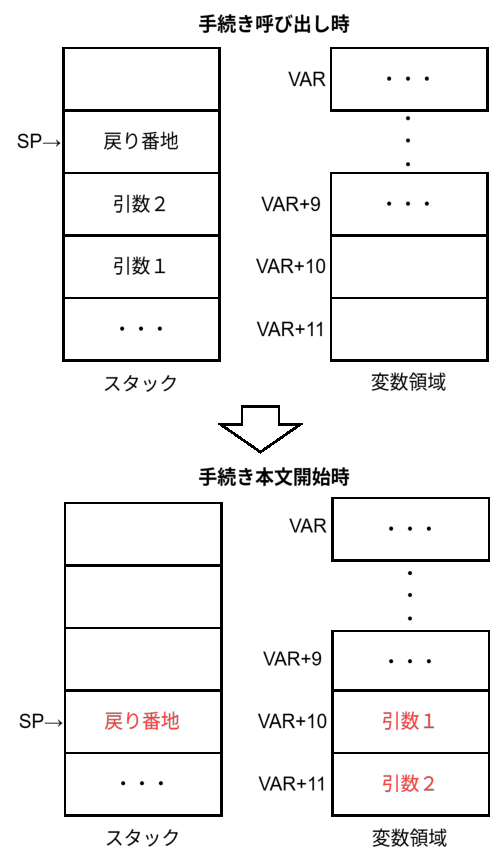
\includegraphics[width=\linewidth]{images/stack.pdf}
    \end{minipage}

    \caption{引数2つの手続きの仮引数処理に伴うスタック操作：プログラム（左）とスタック状態（右）}
    \label{fig:param-callret}
  \end{figure}

  \item \textbf{スコープ管理（識別子表の退避・復元）}\\
  手続き内ではローカル変数・仮引数の登録により識別子表が一時的に拡張されるため，
  \verb|varOffset|・\verb|varKind|・\verb|arrayLower| を手続き生成の開始時に退避し，終了時に復元する．
  これにより，手続き内で追加した識別子が外側へ漏れず，外側の同名識別子の隠蔽も含めて字句的スコープを維持できる．
  図\ref{fig:scope}は，例として\verb|PROC0|が\verb|PROC1|を呼び出したときの識別子表の管理の様子を示したものである．
  呼び出し時に退避，終了時に復元することで，各手続内でのスコープ管理を実現している．
  図からわかるように，\verb|PROC1|呼び出し時には元のスコープ情報を引き継いでそれを拡張し，\verb|PROC1|終了時には\verb|PROC0|は元のスコープ情報を復元する．
  したがって，最終的に\verb|PROC1|はスコープを破棄されるため，呼び出し側の\verb|PROC0|は\verb|PROC1|の情報を保持することなく後続の処理を行うことができる．

  \begin{figure}[htb]
    \centering
    \caption{手続き呼び出し時における，識別子表の退避・復元によるスコープ管理の様子}
    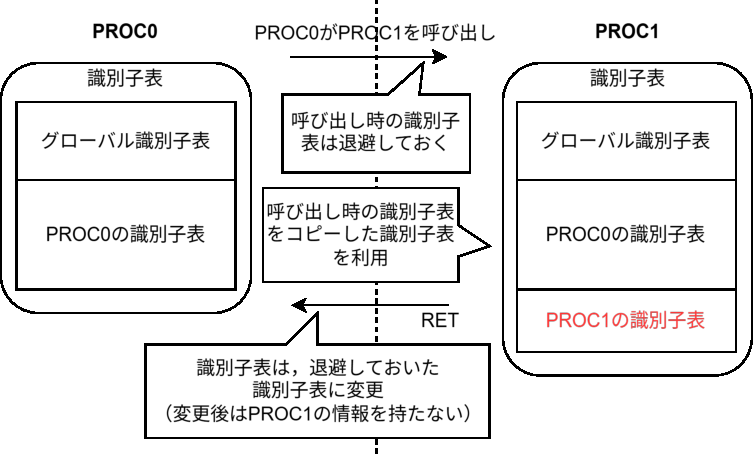
\includegraphics[width=110mm]{images/scope.pdf}
    \label{fig:scope}
  \end{figure}
\end{itemize}


\section{実装プログラム}
\subsection{コード生成器の全体構成}
プログラム\ref{prog:compiler}の \verb|Compiler.run()| は，入力 \verb|ts| の読み込みから構文解析（\verb|AST|生成），意味解析，\verb|CASL| IIプログラム生成，ファイル出力までを順に実行する制御メソッドである．
\verb|TsSource| でトークン列を読み込み，\verb|Syntax.parseProgram()| により \verb|Program| を根とする \verb|AST| を得た後，\verb|Semantic| で宣言・スコープ・型整合性などを検査し，誤りがあればエラーを返して終了する．
問題がなければ \verb|CodeGenerator.generate(ast)| で命令列（\verb|List<String>|）を生成し，\verb|writeCas()| により \verb|cas| へ書き出す．この際，\verb|writeCas()| は \verb|lib.cas| を末尾に連結し，ライブラリルーチンを含む実行可能な\verb|CASL| IIプログラムとして出力する．

一方，\verb|CodeGenerator.generate()| はコード生成本体であり，\verb|emitHeader()| → \verb|ast.accept(this)|（\verb|Visitor|走査）→ \verb|procOut|（手続き定義）→ \verb|emitData()|（\texttt{VAR}/\texttt{CHAR<i>}/\texttt{LIBBUF}）→ \verb|emitFooter()|（\verb|END|）の順に命令列を組み立てて返す．（プログラム\ref{prog:generate}）

なお \verb|ast.accept(this)| 以降は \verb|Visitor| により \verb|AST| を上位ノードから順に走査する．
具体的には \verb|Program| から開始し，まず \verb|Block| 側（変数宣言→手続き宣言の順）を処理した後，最後に \verb|main| 文（複文）を処理する流れである．
このため，領域割当（\verb|visitVarDecl|）や手続きラベル収集・手続き本体生成（\verb|visitProcedureDecl|）を先に完了させた上で，メイン部の命令列が生成される．


\lstinputlisting[caption=\texttt{run}メソッド, firstline=1, firstnumber=1, lastline=21, label=prog:compiler]{codes/compiler.txt}
\lstinputlisting[caption=\texttt{Codegenerator.generate}メソッド, firstline=1, firstnumber=1, lastline=9, label=prog:generate]{codes/generate.txt}

\subsection{データ領域と変数アクセスの実装}
本実装では，変数名と\texttt{VAR}領域上の位置の対応を \verb|varOffset|（\verb|Map<String,Integer>|）に保持している．
具体的には，宣言処理を行う \verb|visitVarDecl| の中で，各識別子 \verb|name| に対して \verb|varOffset.put(name, varCount)| を行い，その時点の \verb|varCount| を「\texttt{VAR}先頭からのオフセット」として登録する．
以後の参照・代入は，必ずこの \verb|varOffset| から得たオフセットに基づいて \texttt{VAR+offset} をアクセスする．

\verb|visitVar|（プログラム\ref{prog:visitVar}）は，プログラム中の左辺変数への代入を\texttt{VAR}領域への書き込みに落とし込む処理である．
まず \verb|lookupOffset(node.name())| により \verb|varOffset| を参照し，識別子名 \verb|node.name()| に対応するオフセット \verb|off| を取得する．
次に \verb|LD GR2, =off| でオフセットを即値として \verb|GR2| に設定する．
右辺値は \verb|visitAssign| が先に \verb|rhs.accept(this)| を実行してスタックへ \verb|PUSH| しているため，
\verb|visitVar| 側では \verb|POP GR1| によりその値を \verb|GR1| に取り出す．
最後に \verb|ST GR1, VAR, GR2| を発行し，\texttt{VAR+off} の1語へ格納することで代入を実現している．

参照側も同様で，\verb|visitVarRef| は同じ \verb|off| を用いて \verb|LD ... VAR, GR2| で読み出し，\verb|PUSH| して式へ返す．
配列は \verb|visitArrayRef/visitArrayAccess| で添字 \verb|i| を評価した後，\verb|k=base-lower|（\verb|base=lookupOffset|，\verb|lower=lookupLower|）で補正し，\verb|ADDA GR2, =k| の後に \verb|LD/ST| を行う．
いずれもアクセスは \texttt{VAR+offset} に統一している．

\lstinputlisting[caption=\texttt{visitVar}メソッド, firstline=1, firstnumber=1, lastline=8, label=prog:visitVar]{codes/visitVar.txt}

\subsection{制御構文と手続き呼出の実装}
\begin{itemize}
  \item \textbf{手続き宣言におけるスコープ管理と出力先の切替}\\
  手続き本体のコード生成では，生成した命令列をメイン部とは別に蓄積するため \verb|currentOut| を \verb|procOut| に切り替え，手続き内でローカル変数・仮引数の登録により識別子表が拡張されるため，\verb|varOffset|・\verb|varKind|・\verb|arrayLower| を退避してから生成し，終了時に復元する．
  これにより，手続き内で追加した識別子が外側へ漏れず，同名識別子の隠蔽を含む字句的スコープをコード生成段階で維持できる．
  出力先の切替と識別子表の退避・復元は，プログラム\ref{prog:procedureDecl}に示すとおりである．
  \lstinputlisting[caption=\texttt{visitProcedureDecl}メソッド, firstline=1, firstnumber=1, lastline=19, label=prog:procedureDecl]{codes/procedureDecl.txt}

  \item \textbf{\texttt{if}/\texttt{while} の展開}\\
  \verb|visitIfS| と \verb|visitWhileS| では，\verb|jumpId| により \texttt{ELSE<i>}・\texttt{ENDIF<i>}・\texttt{LOOP<i>}・\texttt{ENDLP<i>} を一意に採番し，\verb|emit(...)| で分岐命令列を組み立てる．
  条件式は \verb|node.cond().accept(this)| で評価し（結果はスタックに積まれる），\verb|POP| $\rightarrow$ \verb|CPA GR1,=#0000| $\rightarrow$ \verb|JZE| の形で「偽なら分岐」を統一している．
  \texttt{if} は \verb|thenC().accept(this)| で \verb|then| 部を生成し，\texttt{else} があれば \verb|JUMP| で合流点へ飛ばしてから \texttt{ELSE<i>} 側を生成し，最後に \texttt{ENDIF<i>} を置く．
  \texttt{while} は \texttt{LOOP<i>} を先頭に置き，条件が偽なら \texttt{ENDLP<i>} へ分岐し，真なら \verb|body().accept(this)| で本体を生成した後に \verb|JUMP LOOP<i>| で反復を作る．

  \item \textbf{\texttt{CALL} による手続き呼出}\\
  手続き名と入口ラベルの対応は \verb|procLabel|（\verb|Map<String,String>|）で管理する．
  宣言側（\verb|visitProcedureDecl|）で \verb|procLabel.computeIfAbsent(name, n -> "PROC" + (procId++))| により \texttt{PROC<i>} を割り当て，手続き先頭にラベルを出力して入口を確定させる．
  呼出側（\verb|visitProcCall|）では，引数を左から順に \verb|arg.accept(this)| で評価してスタックに積んだ後，\verb|procLabel.get(name)| で宛先ラベルを取得し，\verb|emit("\tCALL\t"+label)| を出力する．
  この方式により，複数の手続き宣言と複数回の呼出に対して，最小限の対応表と採番（\verb|procId|）だけで一意な分岐先を確保できる．
\end{itemize}


\section{考察や工夫点}
\begin{itemize}
  \item \textbf{中間表現（\texttt{AST}）を用いた設計の利点}\\
  本課題では，構文解析で生成した \verb|AST| を中間表現として，意味解析とコード生成の両方で共通利用した．
  ノード種別（\verb|Program, VarDecl, Binary, IfS| など）に対して \verb|Visitor| を適用することで，各処理をノードごとに局所化でき，生成規則の追加・修正が他部分へ波及しにくい構造になった．
  特に，構文（木構造）と処理（意味検査・コード生成）を分離できるため，機能追加やデバッグが容易になった．

  \item \textbf{評価規約の統一（式評価・真偽値・制御構文の共通化）}\\
  式評価は「評価結果をスタックに \verb|PUSH| して親へ返す」という規約に統一し，二項演算は子を先に評価して値を積み，\verb|POP| して演算し，結果を再度 \verb|PUSH| する方式とした．
  また真偽値を \verb|#FFFF|（真）と \verb|#0000|（偽）に正規化し，\verb|if| や \verb|while| では「条件式を評価→\verb|#0000| なら分岐」の形に揃えた．
  この統一により，ネストした式・条件式・比較演算・制御構文を同一の枠組みで展開でき，コード生成の見通しと一貫性が向上した．
  さらに，手続き呼出でも仮引数を \texttt{VAR} へコピーして以後は通常変数と同規約で扱うことで，手続き本体は「スタック＝式評価・一時値用」として自由に利用できる状態を保てるようにした．

  \item \textbf{生成コードの可観測性（コメント付与と段階的検証）}\\
  生成する\verb|CASL| IIコードには，構文要素（代入，\texttt{if}/\texttt{while}，手続き呼出など）に対応したコメントやラベルを付与し，実行時に「どの高級言語構文がどの命令列へ落ちたか」を追跡しやすくした．
  また，\verb|emit| による行単位の蓄積と，ヘッダ／メイン／手続き／データ／フッタの分割出力により，生成結果を部分的に確認しながら段階的にデバッグできるようにした．
  これにより，不具合が生じた場合も，原因箇所（式評価，分岐骨組み，領域参照など）を生成規約の単位で切り分けやすくなった．

  \item \textbf{データ表現とメモリアクセス規約（\texttt{VAR}基準のオフセット設計）}\\
  変数・配列・仮引数をすべて \texttt{VAR} 領域に割り当て，「\texttt{VAR} + \verb|offset|」で参照・代入する規約に統一した．
  \verb|visitVarDecl| で \verb|varOffset| を構築し，配列は \verb|arrayLower| に下限を保持して添字補正（\texttt{base-lower+i}）により連続確保領域へアクセスする．
  文字列定数は \verb|strLabel| で共有し，\texttt{CHAR<i>} ラベルとして \texttt{DC} 領域へ集約することで重複定義を避けた．
  このように参照規約を単純化したことで，コード生成は名前解決と\verb|CASL|命令列生成を明確に分離できた．

  \item \textbf{今後の拡張性（最適化・機能拡張の余地）}\\
  生成器が \verb|AST| を基準に実装されているため，将来的に最適化や機能拡張を差し込みやすい．
  例えば覗き穴最適化として，局所的な命令列をパターンマッチして短縮できる．
  具体例として，\texttt{PUSH 0, GR1} 直後の \texttt{POP GR1} のような無意味な往復の削除，\texttt{LD GR1, =0} に続く \texttt{ADDA GR1, =k} を \texttt{LD GR1, =k} へ畳み込み，\texttt{JUMP L; L NOP} のような冗長ラベルの整理などが考えられる．
  また，将来的にレジスタ割当や定数畳み込み，分岐簡約などを導入する場合も，「\verb|AST|段階の最適化」または「\verb|CASL|出力後の最適化」を独立パスとして追加でき，現行実装を大きく崩さずに性能改善を進められる．
\end{itemize}


\section{感想}
本課題では，字句解析・構文解析・意味解析で得られた情報を用いて，最終的に \texttt{CASL} II の命令列を生成するまでを一貫して実装した．
特に，機能を追加するたびにテストケースを1つずつ確認し，原因を切り分けながら修正していく作業は想像以上に手間がかかり，大変であった．
一方で，小さなテストを積み重ねることで不具合の発生箇所を特定しやすくなり，最終的な安定動作につながることも実感できた．

また，構文解析で作成した \texttt{AST} を中間表現として用い，意味解析とコード生成を \texttt{Visitor} パターンで分離して実装したことで，処理の責務を整理しながら拡張できた点は有用だった．
ノードごとの \texttt{visit} に局所的な規約（スタック規約や \texttt{VAR+offset} 参照規約）を持たせることで，生成規則を追跡しやすく，保守もしやすい構成になったと感じる．

さらに，生成された \texttt{CASL} II アセンブリコードを追いながら動作を確認する過程で，高級言語の構文が条件分岐やスタック操作，データ領域アクセスなどの具体的な命令列に落ちる様子を理解できた．
コンパイラが出力したコードを手で読んで「プログラムが実際にどのように動いているか」を把握する経験は，普段のプログラミングでは得にくい学びであり，今後の低レイヤ理解やデバッグにも役立つと考える．

\end{document}